\documentclass{article}
\usepackage[a4paper, total={6in, 8in}]{geometry}
\usepackage{graphicx}
\usepackage{url}
\usepackage{natbib}
\usepackage{todonotes}
\usepackage{booktabs}
\usepackage{lineno}
\usepackage{color}
%\usepackage{auto-pst-pdf}
\usepackage[colaction]{multicol}
\usepackage{caption}
\usepackage{svg}
\usepackage{authblk}
\usepackage{standalone}
\usepackage[section]{placeins}

\makeatletter
\renewcommand{\maketitle}{\bgroup\setlength{\parindent}{0pt}
	\begin{flushleft}
		
		{\huge\textbf{\@title}}
		
		\bigskip
		
		{\large\textbf{\@author}}
		
		\bigskip
		
		{\large{Draft current \@date}}
		
	\end{flushleft}\egroup
}
\makeatother


\begin{document}
	% Title
	\title{A Topic Model of Climate Change Literature}
	\title{Words, words, words: Mapping the Matter of Climate Change Literature}
	\title{A Topography of Climate Change Research - Methods}
	\author[1,2]{Max Callaghan}
	
	\affil[1]{Mercator Research Institute on Global Commons and Climate Change, Torgauer Straße, 10829 Berlin, Germany}
	\affil[2]{School of Earth and Environment, University of Leeds, Leeds LS2 9JT, United Kingdom}
	\maketitle
	\begin{linenumbers}
	
	\setcounter{figure}{0}
	\renewcommand\thefigure{SI.\arabic{figure}}  
		
	\subsection*{Data}
	
	This study reproduces the query developed by \citep{Grieneisen2011}, which is carried out on the Web of Science core collection. Though not exhaustive, the Web of Science gives a good coverage of the literature in major peer-reviewed journals. The Web of Science data gives us a disciplinary classification (based on the journal) and publication year, among other metadata, for each document.	Each document is assigned to an assessment period according to the timeline shown in table 1.
	
	We use the references scraped from IPCC assessment reports from \citep{Minx2017l}, and attempt to match these with the results from the Web of Science. We use doc2vec similarity scores \cite{Le2014} to identify the 500 most similar titles for each reference, and count the document as a match if the jaccard similarity score of the two word shingles of the reference title and the document title is greater than 0.5 \cite{Khabsa2014}. Table \ref{ipcc-matching} shows the percentage of IPCC citations matched in each working group for each assessment report. This is significantly lower in earlier periods, as data coverage and quality of citation databases is lower for earlier periods. Matching in WG III is also lower, suggesting a greater share of non-peer review literature, or literature not directly mentioning climate change, but related to it's mitigation (for example on energy policy).
	
		\begin{table}[htp]
			\begin{center}
		\begin{tabular}{lrrrrr}
\toprule
AR &  1 &   2 &   3 &   4 &   5 \\
WG &    &     &     &     &     \\
\midrule
1  & 8\% & 25\% & 37\% & 47\% & 58\% \\
2  & 6\% & 12\% & 30\% & 38\% & 47\% \\
3  & 3\% &  9\% & 15\% & 22\% & 35\% \\
\bottomrule
\end{tabular}

	\caption{IPCC matching}
	\label{ipcc-matching}
	\end{center}
\end{table}
	
		
	\subsection*{Pre-processing}
	
	Data quality in earlier Web of Science results is poorer, and some documents have missing abstracts. In the quantification of the size of the literature and its vocabulary in table \ref{tab}, titles are substituted for abstracts where they are not available.  The words of the documents are lemmatized, replacing different forms of the same word (i.e. word/words) with a single instance. Commonly occurring words, or ``stopwords'' are removed, as are all words shorter than 3 characters, and all words containing only punctuation or numbers.
	
	The documents are transformed into a document-term matrix, where each row represents a document, and each column represents a unique word.  Each cell contains the number of that column's terms in that document. Only terms which occur more than once are considered.
	
	For the calculation of the topic model, documents with missing abstracts are ignored, and the document term matrix is transformed into a document
	frequency-inverse document frequency (tf-idf) matrix, where scores are scaled according to the frequency of their occurrence in the corpus. This gives more weight to terms which appear in few documents, and less weight to those which appear in many.
	
	\begin{equation}
	tf(t,d) = f_{t,d} \mathrm{,}\quad idf(t,D) = \log\frac{N}{|\{d \in D:t \in d\}|}
	\end{equation} 
	
	\subsection*{Topic Model}
	
	We use non-negative Matrix Factorisation (NMF) \cite{Lee1999}, an approach to topic modelling which factorises the term-frequency-inverse document frequency matrix \( V \) into the matrices \(W\), the topic-term matrix, and \( H \) the document-topic matrix, whose product approximates \(V\):
	
	\begin{equation}
		V_{i\mu} \approx (WH)_{i\mu} = \sum_{a=1}^{r}W_{ia}H_{a\mu}
	\end{equation}
	
	As demonstrated in Figure \ref{doc-topic}, each topic is represented as a set of word scores, and each document a set of topic scores. The combination of the two give the word scores in the document. For clarity in the figure, these are shown as simple counts, but in the model these are scaled according to each term's frequency within the corpus as explained above.
	
	Topics are calculated using the scikitlearn library \cite{Pedregosa2011}, and are saved in a database and topic visualisation system based on \cite{Chaney2012} \footnote{The system adds new functionality to \cite{Chaney2012} and combines it with a system for managing sets of documents and queries. The code and additional information is published online at \url{https://github.com/mcallaghan/tmv}}. 	
	
	\subsubsection*{Model selection}
	
	Topic models are calculated for 70, 80, 90, 100, 110, 120, 130, 140 and 150 topics. The run with 150 topics was discarded as it contained a topic to which no terms or documents were assigned. The relative usefulness of each model was assessed subjectively by the authors, based on inspection of the online visualisation tool, and the spreadsheet \textbf{topic\_comparison.xlsx} accompanying the supporting information. The spreadsheet shows each set of topics in adjacent columns. Topics from each model are placed next to the topics with the largest number of each topic's 10 highest scoring words in common. This helps authors to find an appropriate level of granularity for the analysis. 
			
	\subsubsection*{Topic Representation and Newness}
	
	To calculate topic representation in IPCC reports we divide each topic's share in the subsample of documents cited by IPCC reports by its share in the whole corpus. 
	
	We calculate a topic's total score as the sum of document-topic scores. A topic's window score is the sum of document-topic scores considering only documents in the given time window. To represent a topic's newness, we multiply each assessment period number by the share of it's total score occurring in that window, and take the mean of these scores. A topic in which 100\% of documents which make it up occurred in assessment period 1 (6) would thereby receive a score of 1 (6), while a topic evenly distributed across all assessment periods would receive a score of 3.5.
	
	
	\subsubsection*{Disciplinary Entropy}
	
	Disciplinary Entropy inverts the measurement of a conference's topical diversity suggested in \cite{Hall2008}, by measuring a topic \(z\)'s entropy \(H\), where 
	
	\begin{equation}
		H(f|z) = -\sum_{i=1}^K \hat{p}(f|z) \log \hat{p}(f|z) 
	\end{equation}
	
	based on the empirical distribution of a field \(f\) in the documents \(d\) in each topic:
	
	\begin{equation}
		\hat{p}(f|z) = \sum_{d:z_d=z} \hat{p} (f|d) \hat{p} (d|z)
	\end{equation}
	
	\subsubsection*{Topic Map}
	The topic model gives us the location of each document in a 140 dimensional topic space, with each dimension corresponding to a that document's \textit{topic-ness} in a given topic. t-Distributed Stochastic Neighbour Embedding (t-SNE) is a dimensionality reduction technique which we use to represent each document's topic scores in 2 dimensions \cite{vandermaaten2008}.

	\begin{figure}
		\begin{center}
			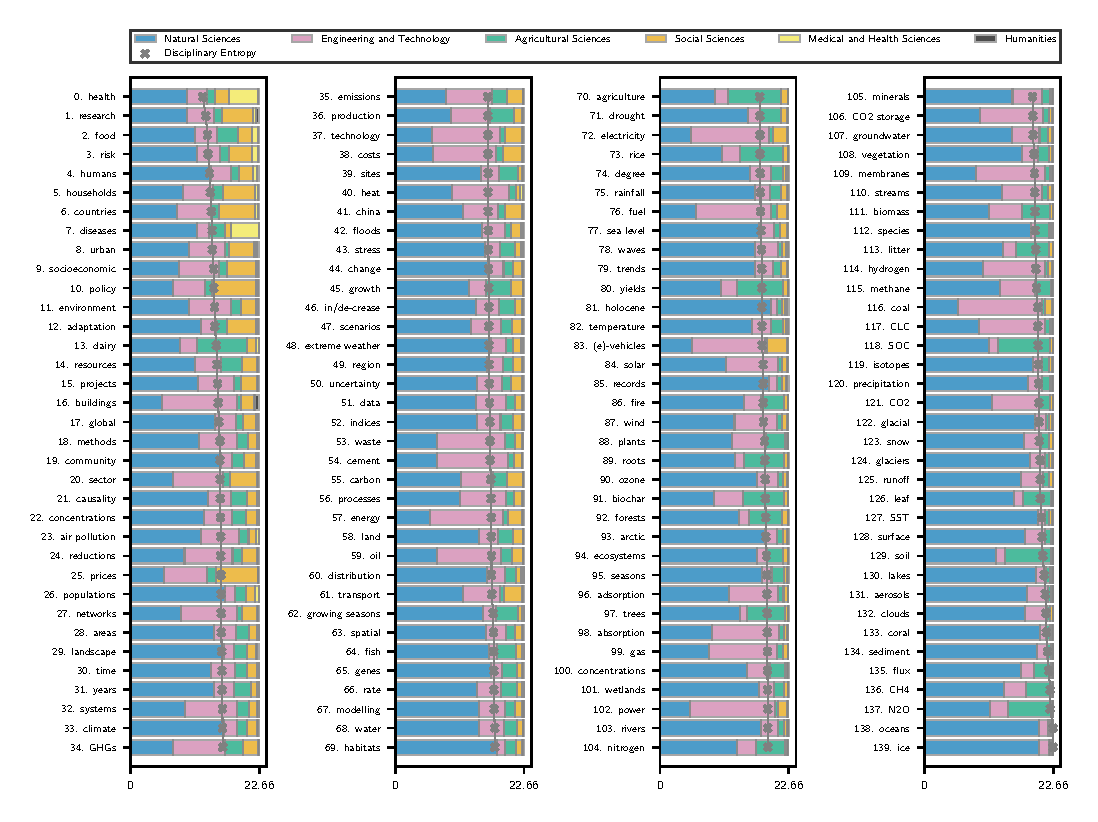
\includegraphics[width=1\linewidth]{plots_pub/topic_oecd_entropy.pdf}
			\caption{SI Disciplinary Entropy}
			\label{dis-entropy}
		\end{center}
	\end{figure}	
	
	
	
	\begin{figure}
		\begin{center}
			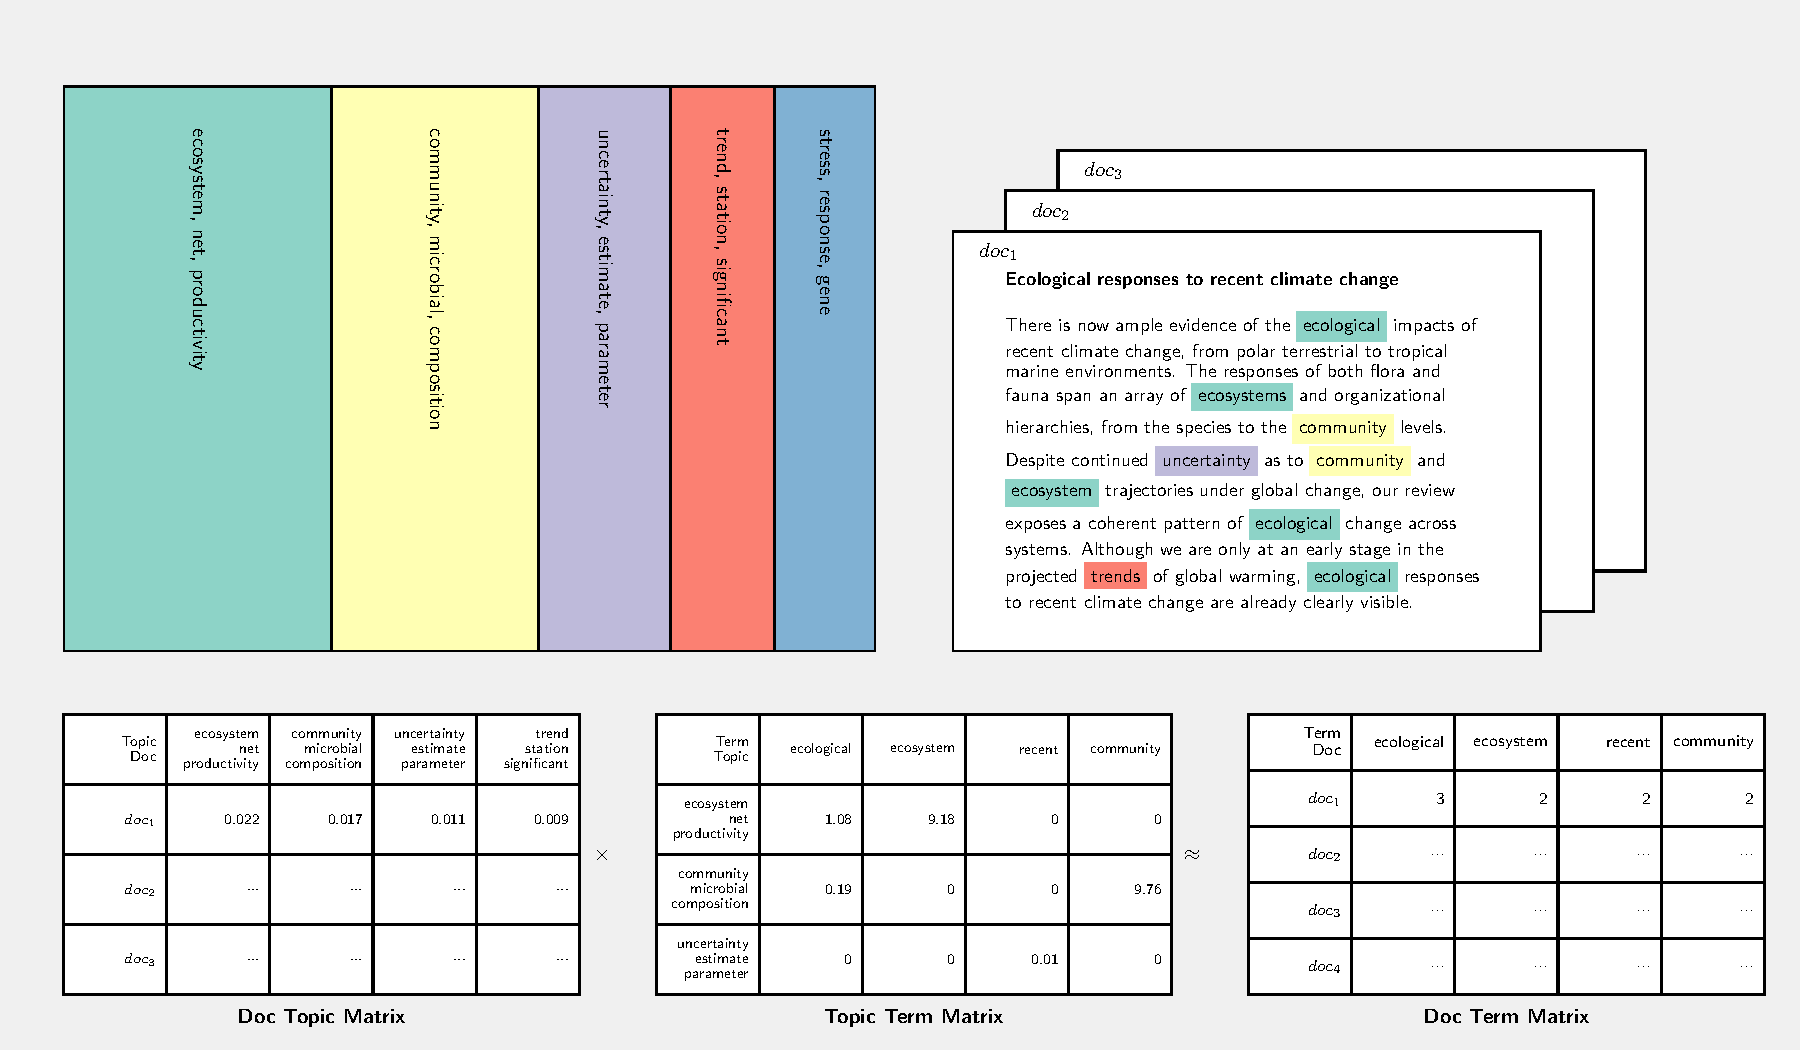
\includegraphics[width=1\linewidth]{plots_pub/single_doc_3_536594_1861.pdf}
			\caption{SI Topic make up of a single document}
			\label{doc-topic}
		\end{center}
	\end{figure}

	\begin{figure}
	\begin{center}
		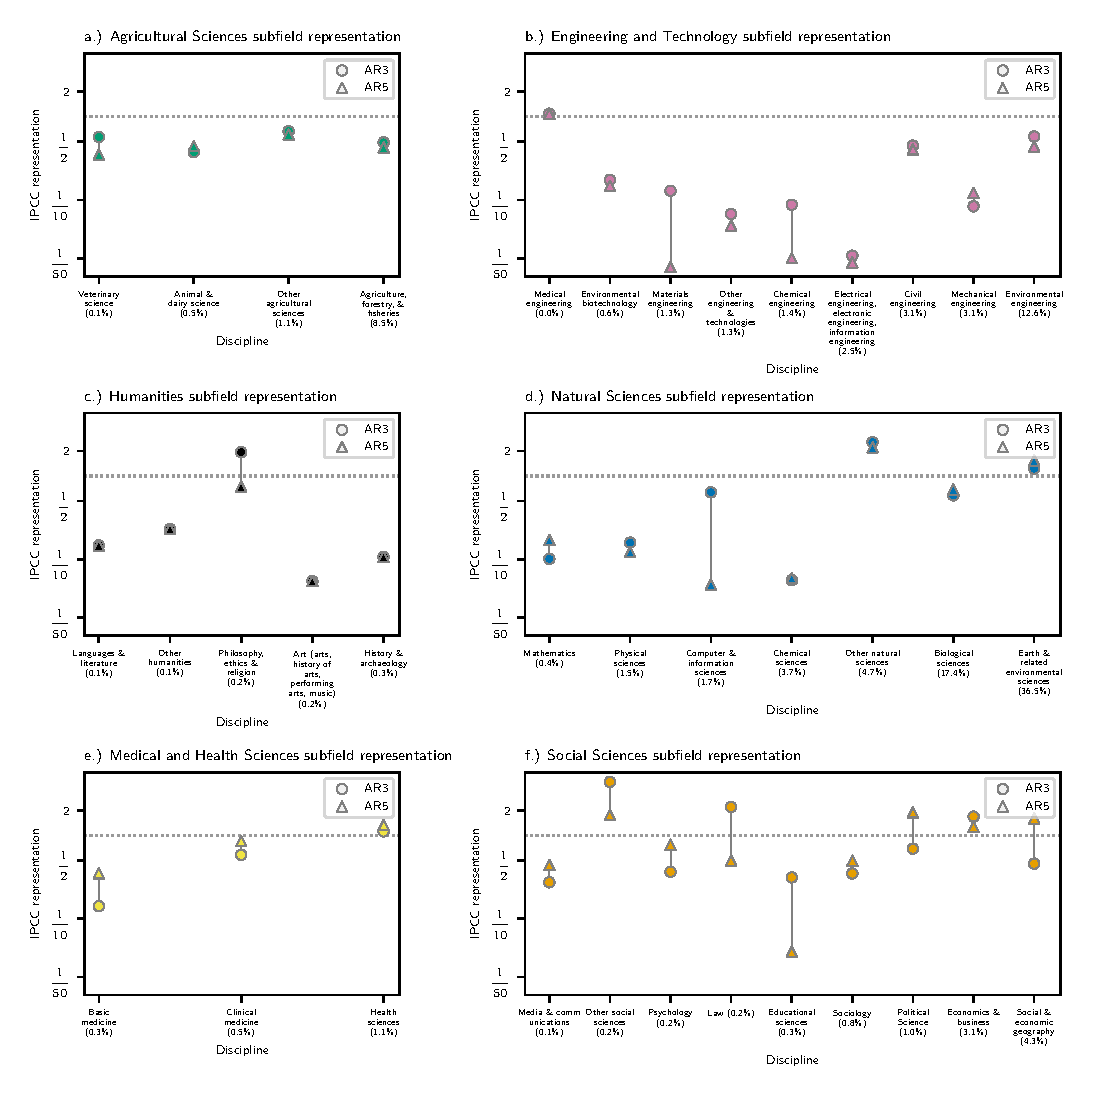
\includegraphics[width=1\linewidth]{plots_pub/ipcc_rep_wcs_simplified.pdf}
		\caption{SI Representation by subfield}
		\label{subfield}
	\end{center}
\end{figure}

\begin{figure}
	\begin{center}
		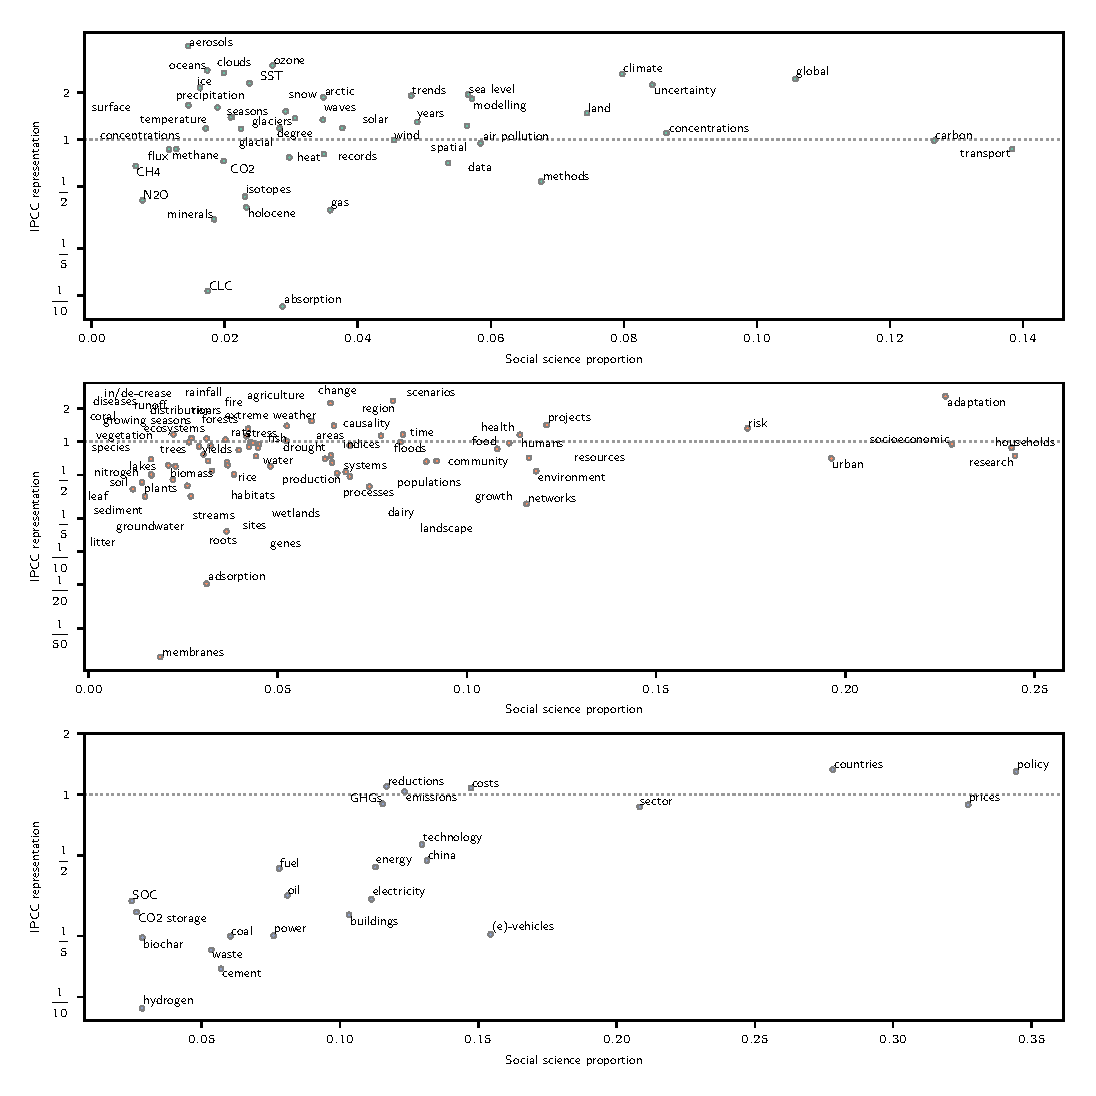
\includegraphics[width=1\linewidth]{plots_pub/wgs_socsci.pdf}
		\caption{SI Social science \& representation in topics across working groups}
		\label{socsci-wgs}
	\end{center}
\end{figure}

\begin{figure}
	\begin{center}
		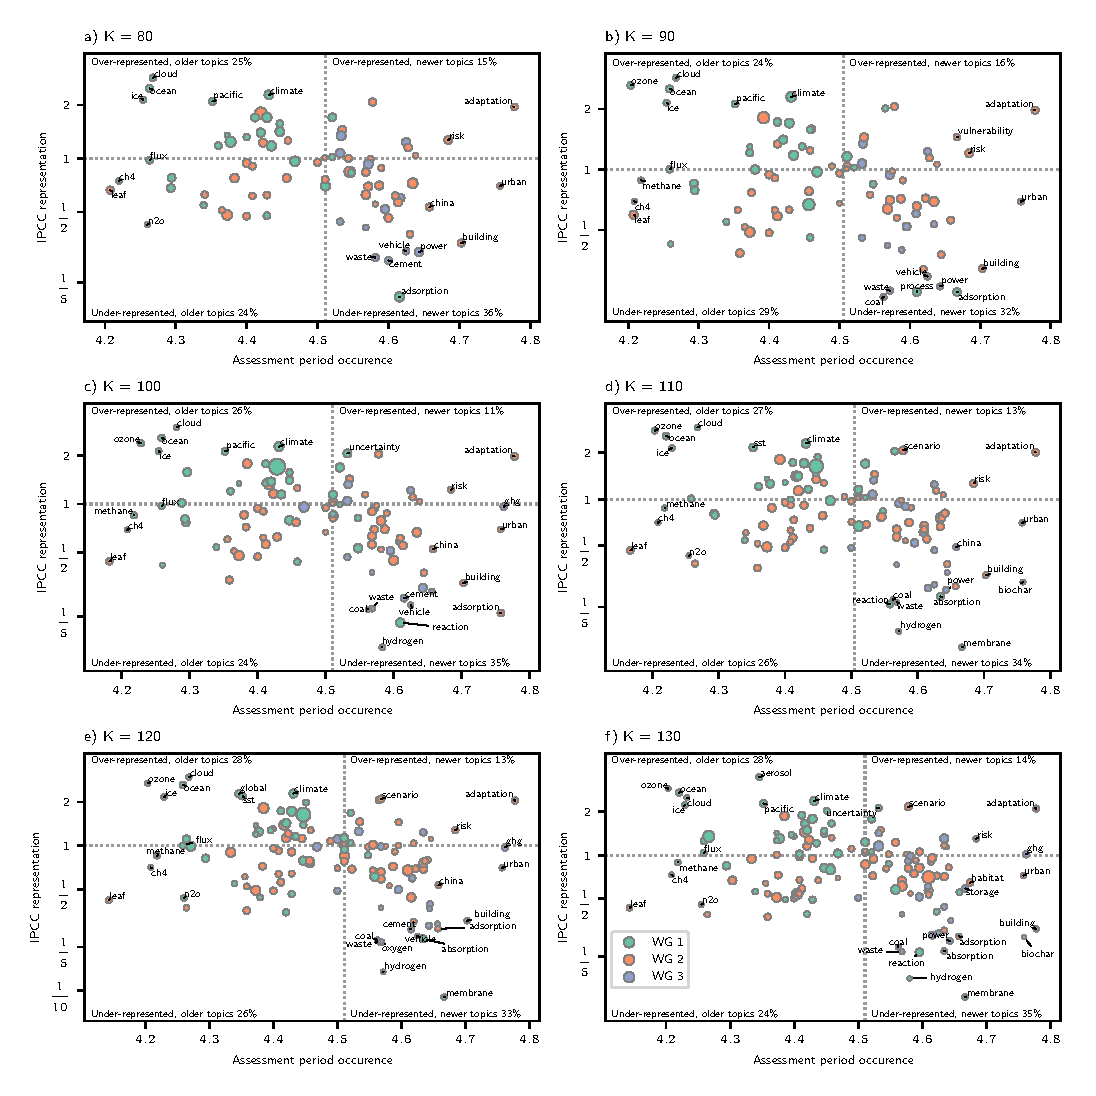
\includegraphics[width=1\linewidth]{plots_pub/topic_rep_ks.pdf}
		\caption{Topic representation over different values of K (number of topics). Topics in the upper or lower 6.66th percentile of either dimension are labelled}
		\label{top-rep-ks}
	\end{center}
\end{figure}

\subsection*{Glossary}


\noindent\textbf{ncep:} National Centers for Environmental Protection

\noindent\textbf{fco:} Fugacity of Carbon Dioxide

\noindent\textbf{pfc:} Perflourocompound

\noindent\textbf{otcs:} Open Top Chambers

\noindent\textbf{dtr:} Diurnal Temperature Range

\noindent\textbf{sres:} Special Report on Emissions Scenarios (200)

\noindent\textbf{petm:} Paleocene Eocene Thermal Maximum

\noindent\textbf{amf:}  Arbuscular Mycorrhizal Fungal

\noindent\textbf{sf5cf3:} trifluoromethyl sulfur pentafluoride (A Potent Greenhouse Gas Identified in the Atmosphere, 2000)

\noindent\textbf{clc:} Chemical Looping Combustion

\noindent\textbf{cwd:} Coarse woody debris

\noindent\textbf{etm:} Enhanced Thematic Mapper (NASA satellite sensor)

\noindent\textbf{cmip5:} Coupled Model Intercomparison Project 5 (Starting 2008)

\noindent\textbf{cmip3:} Coupled Model Intercomparison Project phase 3 (first published 2007 \cite{Meehl2007})

\noindent\textbf{mofs:} metal-organic frameworks (for CO2 storage)

\noindent\textbf{sdm:} statistical-dynamical model

\noindent\textbf{mmms:} Mixed Matrix Membranes (for CO2 capture)

\noindent\textbf{cop21:} 21st Conference of Parties (Paris 2015) 

\noindent\textbf{c3n4:} Carbon nitride (a synthetic nanomaterial used for hydrogen production)

\noindent\textbf{sdg:} Sustainable Development Goals

\noindent\textbf{indc:} Intended Nationally Determined Contributions

		
	\end{linenumbers}

\linespread{1}

%\bibliography{Mendeley}

\begin{thebibliography}{10}
	
	\bibitem{Grieneisen2011}
	Michael Grieneisen and Minghua Zhang.
	\newblock {The Current Status of Climate Change Research}.
	\newblock {\em Nature Climate Change}, 1:72--73, 2011.
	
	\bibitem{Minx2017l}
	Jan~C. Minx, Max Callaghan, William~F. Lamb, Jennifer Garard, and Ottmar
	Edenhofer.
	\newblock {Learning about climate change solutions in the IPCC and beyond}.
	\newblock {\em Environmental Science {\&} Policy}, 2017.
	
	\bibitem{Le2014}
	Quoc~V. Le and Tomas Mikolov.
	\newblock {Distributed Representations of Sentences and Documents}.
	\newblock {\em ICML}, 32, 2014.
	
	\bibitem{Khabsa2014}
	Madian Khabsa and C~Lee Giles.
	\newblock {The number of scholarly documents on the public web}.
	\newblock {\em PLoS ONE}, 9(5), 2014.
	
	\bibitem{Lee1999}
	D~D Lee and H~S Seung.
	\newblock {Learning the parts of objects by non-negative matrix factorization.}
	\newblock {\em Nature}, 401(6755):788--791, 1999.
	
	\bibitem{Pedregosa2011}
	Fabian Pedregosa, Ga{\"{e}}l Varoquaux, Alexandre Gramfort, Vincent Michel,
	Bertrand Thirion, Olivier Grisel, Mathieu Blondel, Peter Prettenhofer, Ron
	Weiss, Vincent Dubourg, Jake Vanderplas, Alexandre Passos, David Cournapeau,
	Matthieu Brucher, Mattheiu Perrot, and {\'{E}}douard Duchesnay.
	\newblock {Scikit-learn: Machine Learning in Python Fabian}.
	\newblock {\em Journal of Machine Learning Research}, 12:2825--2830, 2011.
	
	\bibitem{Chaney2012}
	Allison J~B Chaney and David~M. Blei.
	\newblock {Visualizing Topic Models}.
	\newblock {\em Icwsm}, pages 419--422, 2012.
	
	\bibitem{Hall2008}
	David Hall, Daniel Jurafsky, and Christopher~D. Manning.
	\newblock {Studying the history of ideas using topic models}.
	\newblock {\em Proceedings of the Conference on Empirical Methods in Natural
		Language Processing - EMNLP '08}, pages 363--371, 2008.
	
	\bibitem{vandermaaten2008}
	Laurens van~der Maaten and Geoffrey Hinton.
	\newblock {Visualizing Data using t-SNE}.
	\newblock {\em Journal of Machine Learning Research}, 9:2579--2605, 2008.
	
	\bibitem{Meehl2007}
	Gerald~A. Meehl, Curt Covey, Thomas Delworth, Mojib Latif, Bryant McAvaney,
	John~F.B. Mitchell, Ronald~J. Stouffer, and Karl~E. Taylor.
	\newblock {The WCRP CMIP3 multimodel dataset: A new era in climatic change
		research}.
	\newblock {\em Bulletin of the American Meteorological Society},
	88(9):1383--1394, 2007.
	
\end{thebibliography}

\bibliographystyle{unsrt}

\end{document}